%% Draft settings
\documentclass[10pt]{article}
\usepackage{amsmath}
\usepackage{amssymb}
\usepackage{graphicx}
\usepackage{subfigure}
\usepackage{color}
 \usepackage{lineno}
\usepackage{simplemargins}
\usepackage{natbib}

% \linenumbers*[1]
 \usepackage[T1]{fontenc} % For citing barki{\dj}ija
\setkeys{Gin}{draft=false}


% Margins
\setleftmargin{1in}
\setrightmargin{1in}
\setbottommargin{1in}
\settopmargin{1in}
 

% Standard shortcuts
\input{/Users/nadir/Dropbox/resources/shortcuts.tex}

% radiation shorthand
\newcommand{\QLW}{\ensuremath{Q_\mathrm{LW}}}
\newcommand{\QSW}{\ensuremath{Q_\mathrm{SW}}}
\newcommand{\Qnet}{\ensuremath{Q_\mathrm{net}}}
\newcommand{\Qcts}{\ensuremath{Q_\mathrm{cts}}}
\newcommand{\Qgex}{\ensuremath{Q_\mathrm{gex}}}
\newcommand{\FLW}{\ensuremath{F}}
\newcommand{\FSW}{\ensuremath{F^\mathrm{SW}}}
\newcommand{\Fnet}{\ensuremath{F^\mathrm{net}}}
\newcommand{\trans}{\ensuremath{\mathcal{T}}}
\newcommand{\cool}{\ensuremath{\mathcal{C}}}
\newcommand{\ch}{\ensuremath{\mathcal{H}}}
\newcommand{\chk}{\ensuremath{\ch_k}}
\newcommand{\chcts}{\ensuremath{\mathcal{H}^\CTS}}
\newcommand{\chkcts}{\ensuremath{\ch_k^\CTS}}
\newcommand{\pierre}{P10}
\newcommand{\pem}{\ensuremath{p_1}}
\newcommand{\lk}{\ensuremath{l_k}}
\newcommand{\lj}{\ensuremath{l_j}}
\newcommand{\tauk}{\ensuremath{\tau_k}}
\newcommand{\tauks}{\ensuremath{\tau_{k,s}}}
\newcommand{\taus}{\ensuremath{\tau_s}}
\newcommand{\tautilde}{\ensuremath{\tilde{\tau}}}
\newcommand{\Bs}{\ensuremath{B_s}}
\newcommand{\SX}{\ensuremath{\mathrm{SX}}}
\newcommand{\AX}{\ensuremath{\mathrm{AX}}}
\newcommand{\GX}{\ensuremath{\mathrm{GX}}}
\newcommand{\CTS}{\ensuremath{\mathrm{CTS}}}
\newcommand{\EXbelow}{\ensuremath{\mathrm{EX_{below}}}}
\newcommand{\EXabove}{\ensuremath{\mathrm{EX_{above}}}}
\newcommand{\mubar}{\ensuremath{\bar{\mu}}}
\newcommand{\kapparef}{\ensuremath{\kappa_{\mathrm{ref}}}}
\newcommand{\kappao}{\ensuremath{\kappa_0}}
\newcommand{\Tref}{\ensuremath{T_{\mathrm{ref}}}}
\newcommand{\pref}{\ensuremath{p_{\mathrm{ref}}}}
\newcommand{\WVP}{\ensuremath{\mathrm{WVP}}}
\newcommand{\Tav}{\ensuremath{T_{\mathrm{av}}}}
\newcommand{\Tstrat}{\ensuremath{T_{\mathrm{strat}}}}



% kappa param variables
\newcommand{\kapparot}{\ensuremath{\kappa_{\mathrm{rot}}}}
\newcommand{\kappavr}{\ensuremath{\kappa_{\mathrm{vr}}}}
\newcommand{\kappaQ}{\ensuremath{\kappa_Q}}
\newcommand{\krot}{\ensuremath{k_\mathrm{rot}}}
\newcommand{\kvr}{\ensuremath{k_\mathrm{vr}}}
\newcommand{\konerot}{\ensuremath{k_{1\mathrm{rot}}}}
\newcommand{\konevr}{\ensuremath{k_{1\mathrm{vr}}}}
\newcommand{\kQ}{\ensuremath{k_Q}}
\newcommand{\koneP}{\ensuremath{k_{1P}}}
\newcommand{\koneR}{\ensuremath{k_{1R}}}
\newcommand{\konej}{\ensuremath{k_{1j}}}
\newcommand{\lrot}{\ensuremath{l_\mathrm{rot}}}
\newcommand{\lvr}{\ensuremath{l_\mathrm{vr}}}
\newcommand{\lQ}{\ensuremath{l_{Q}}}
\newcommand{\vr}{\ensuremath{\mathbf{vr}}}
\newcommand{\rot}{\ensuremath{\mathbf{rot}}}


%Variables
\newcommand{\figurepath}{../figures/}


\begin{document}

%% ------------------------------------------------------------------------ %%
%
%  TITLE
%
%% ------------------------------------------------------------------------ %%


\title{On the cooling-to-space from water vapor and carbon dioxide}

%% ------------------------------------------------------------------------ %%
%
%  AUTHORS AND AFFILIATIONS
%
%% ------------------------------------------------------------------------ %%


 \author{Nadir Jeevanjee and Stephan Fueglistaler}

\maketitle

\begin{abstract}
Although spectral greenhouse gas radiative transfer is in principle well-understood, an intuitive understanding of its phenomenology is often lacking. In particular, it is unclear why tropospheric radiative cooling is roughly 1 K/day, or why the contributions to this from carbon dioxide are an order of magnitude smaller than that from water vapor.

One avenue for such understanding is the cooling-to-space (CTS) approximation, which despite being well known has not been properly justified, nor fully exploited as a tool for understanding. Here we investigate the CTS approximation in detail, and analyze why it works well for water vapor but less so for for carbon dioxide. We obtain cooling rates from the Reference Forward Model, a comprehensive line-by-line radiative transfer model, and decompose these cooling rates into the CTS term plus other contributions using an offline code. We also gain intuition for the CTS approximation with some simple analytical theory.

Finally, we apply the CTS approximation along with simplified spectroscopy to obtain analytical expressions for the radiative cooling from water vapor and carbon dioxide. These expressions reproduce the observed 1 K/day cooling rate, and express it as a product of the Planck function, an optical depth scale height, and a characteristic spectral width.



%\vspace{0.5cm}
%
%
\end{abstract}


%% ------------------------------------------------------------------------ %%
%
%  TEXT
%
%% ------------------------------------------------------------------------ %%


\section {Introduction}
Despite its fundamental role in driving atmospheric motions, atmospheric radiative cooling remains somewhat enigmatic. Though the fundamentals of radiative transfer are quite well-understood and have been for some time, translating these fundamentals into realistic cooling rates requires complicated radiative transfer calculations which render the final result somewhat inscrutable. As a result, we lack simple descriptions of the radiative cooling profiles produced by our numerical models. For example, Fig. \ref{coo_tau_kappa_h2o}a shows the heating rate
\beqn
	\ch \ \equiv \ \frac{g}{\Cp} \ppp F \quad \text{(K/day)}
	\label{heat}
\eeqn
as computed by the RFM line-by-line radiative transfer model \citep{dudhia2017} for an idealized atmosphere with surface temperature $\Ts=300$ K, a constant lapse rate of $\Gamma= 7\ \Kelvin/\km$ up to to an isothermal stratosphere at $\Tstrat=200$ K, and \htwo\ as the only radiatively active species  with  \RH=0.75. Here $F$ is the net upward longwave (LW) flux, in \Wmsq, and further details on the RFM calculation can be found in section \ref{sec_cts_lbl}. The heating is roughly $-2$ K/day, a typical number. But, what physics determines this number? In particular, can it be estimated in a back-of-the-envelope fashion, or can it only be determined by a comprehensive radiative transfer calculation like the one performed here?

Since \ch\ is calculated by integrating the spectrally-resolved heating 
\beqn
	\ch_k \ \equiv \ \frac{g}{\Cp} \ppp F_k \quad \text{(K/day/\cminverse)}
	\label{heat_k}
\eeqn
(where $k$ denotes wavenumber and $F_k$ is spectrally-resolved flux in $\Wmsq/\cminverse$),  any understanding of \ch\ must stem from an understanding of \chk, which we plot in Fig. \ref{coo_tau_kappa_h2o}b.  The broad structure of $\ch_k$, with two diagonal bands of cooling in $k-p$ space, can be understood in terms of the optical depth
\beqn
	\tauk(p) \ \equiv  \ \int_0^p \, \underbrace{\kappa(k,T,p')}_{\meter^2/\kg} \underbrace{q \frac{dp'}{g}}_{\kg/\meter^2}\ .
	\label{tauk}
\eeqn
Here $q$ is the specific concentration of our greenhouse gas and $\kappa$ is the wavenumber-dependent mass absorption coefficient ($\meter^2/\kg$), which also depends on $T$ and $p$  due to temperature-scaling and pressure broadening \citep[][hereafter P10]{pierrehumbert2010}. All other symbols have their usual meaning. Note that since $\kappa$ is an effective area per unit mass, and the rest of the integrand in \eqnref{tauk} is just the mass per unit area of absorber above level $p$ (i.e. the path length), $\tauk$ can be interpreted as the effective area of absorbers above level $p$ per unit (geometric) area.

 Optical depth as output from RFM is shown in Fig. \ref{coo_tau_kappa_h2o}c, which also plots the $\tauk=1$ levels for each $k$. The two diagonal bands in the \chk\ plot correspond to two diagonal $\tauk=1$ bands, which is where we expect emission at a given $k$ to maximize \citep[e.g.][hereafter P06; we discuss the basis for this `$\tau=1$' law below]{petty2006}. The shape of these $\tauk=1$ bands can themselves be understood in terms of reference absorption coefficients 
 \beqn
  \kapparef(k)\ \equiv  \ \kappa(k,\Tref,\pref)
  \eeqn
  where we take $(\Tref,\pref)=(300\ \Kelvin, 1\ \text{atm})$. These coefficients, also output from RFM, are shown in  Fig. \ref{coo_tau_kappa_h2o}d. The two $\tauk=1$ bands  in Fig. \ref{coo_tau_kappa_h2o}c correspond to the two absorption bands evident in the \kapparef\ plot: the pure rotation band ($k < 1000\ \cminverse$), and vibration-rotation band ($1000 < k< 1450 \ \cminverse$). By \eqref{tauk}, where \kapparef\ is relatively large then $\tauk=1$  occurs at relatively low pressures,  and vice-versa, so that plots of \kapparef\ and $\tauk=1$ levels must necessarily have the same shape. 

This description of \chk, while not standard in textbooks, can be found in the literature \citep[e.g.][]{clough1992}. The $\tau=1$ law that we invoked, however, strictly speaking applies only to the emission of OLR (or `cooling-to-space'), not radiative heating rates \emph{per se}; this is because  the latter includes not just cooling-to-space but also radiative exchange between atmospheric layers as well as the surface. That the $\tau=1$ law evidently applies to heating rates also (Fig. \ref{coo_tau_kappa_h2o}) then suggests that these exchange terms may be negligible, leading to the  \emph{cooling-to-space approximation} (e.g. P06, section 10.4):  
\beqn
	\ppp F_k \ \approx \   \pi B(k,T) \partialder{\trans_k}{p} \  .
	\label{cts}
\eeqn
Here $\trans_k \ \equiv \ \exp(-\tauk)$ is the transmission function and $\pi B(k,T) \partialder{\trans_k}{p}$ is the cooling-to-space (or CTS) term in pressure coordinates, representing the differential contribution of an atmospheric layer to the \OLR\ at wavenumber $k$. In the CTS approximation then, radiative flux divergence is  simply Planck emission $\pi B(k,T)$ times a transmissivity gradient, the latter of which also serves as a weighting function since for optically thick wavenumbers its characteristic width and magnitude are constrained by $\int\ppp\trans_k \, dp = 1$. That the CTS term maximizes at $\tau=1$ is suggested by writing this transmissivity gradient as 
 \beqn
 	\partialder{\trans_k}{p} \ = \ -\partialder{\ln \tauk}{p} \tauk e^{-\tauk} \ .
	\label{trans_grad}
\eeqn
 The function $\tauk \exp(-\tauk)$ has a relatively sharp peak at $\tauk=1$, and so long as \partialder{\ln\tauk}{p}  has negligible vertical structure in the neighborhood of $\tau=1$, the transmissivity gradient and hence the CTS term will peak 
at $\tau=1$. Note also that \partialder{\ln\tauk}{p}\ is an inverse  `scale pressure' for optical depth, measuring how quickly \tauk\ increases by one $e$-folding, and that it simultaneously determines the width and magnitude of the transmissivity gradient. This quantity will play a key role in later sections.

Returning to heating rates, we now plot \chcts\ and \chkcts, the spectrally integrated and resolved heating rates calculated using  \eqnref{cts},  in Fig. \ref{coo_tau_kappa_h2o}a,b. Away from the surface, the CTS approximation appears to be quite accurate, as noted by previous studies \citep[e.g.][]{clough1992,rodgers1966}.  In addition, the \CTS\ term has a very simple mathematical structure,  and unlike the exact spectral cooling \eqref{heat_k} does not require an integration of the radiative transfer equations to find $F_k$. The \CTS\ term is thus much simpler to compute and manipulate than the total cooling, an advantage utilized by some GCM radiation parameterizations  \citep[e.g.][]{fels1980}.

The narrative so far ties together various pieces of radiative transfer physics in a satisfying way: spectrally-resolved heating rates \chk\ are dominated by the \CTS\ term \chkcts, which maximizes where $\tauk=1$, the height  of which is determined by \kapparef.  At the same time, however, this narrative does not yet provide a back-of-the-envelope estimate of \ch. Also, we still lack an understanding of why the \CTS\ approximation works so well, and under what conditions we might  expect it to break down.

To bring these questions into focus,  Fig. \ref{coo_tau_kappa_co2} shows plots analogous to that of Fig. \ref{coo_tau_kappa_h2o}, with the same idealized atmosphere except with \cotwo\ rather than \htwo\ as the radiatively active species, with a \cotwo\ concentration of 280 ppmv. The narrative of the previous paragraph largely holds, in that the bands of cooling correspond to $\tauk=1$ levels which themselves are determined by $\kapparef(k)$,  but some differences with the \htwo-only case emerge. Firstly, the mid-tropospheric spectrally integrated heating \ch\ for \cotwo\ is several  times smaller in magnitude than that for \htwo. Though this seems largely due to the width of their respective absorption bands, it is unclear how to make this  quantitative. Furthermore, the widths of these bands cannot be the whole story, as the spectrally-\emph{resolved} heating rates \chk\ for \cotwo\ are roughly half that of \htwo.  Finally, Fig. \ref{coo_tau_kappa_co2}a-c shows that the \CTS\ approximation holds less well for \cotwo\ than for \htwo. The reasons for this are unclear, as to date the CTS approximation seems only to have been justified by numerical experiment, rather than theoretical analysis. 

This review of the physics of radiative cooling has thus raised several questions:
\begin{enumerate}
	\item Why is $\ch\sim O(1\ \text{K/day})$? Can this be estimated in a back-of-the-envelope fashion? \label{Q_heating}
	\item Why does the CTS approximation work, and why does it work better for \htwo\ than \cotwo?	    \label{Q_cts}
	\item Why is $\ch_k$ twice as large for \htwo\ as for \cotwo, and why is \ch\ several times larger?		\label{Q_contrast}
\end{enumerate}

The goal of this paper is to answer these questions, by building and using simple radiation models which nonetheless emulate much more comprehensive radiative transfer schemes \citep[see][for further discussion of this approach]{jeevanjee2017a}. Our first task will be to understand the radiative cooling from a single spectral line (Section \ref{sec_single_line}); we do this in both a gray gas and real gas context , with the \CTS\ approximation playing a leading role in both. This single line analysis will yield answers to question \ref{Q_cts}. We then tackle the full spectrum of real gas radiation in Section \ref{sec_cts_theory}, where we combine the \CTS\ approximation with a parameterization of greenhouse gas spectroscopy inspired by that of \cite{wilson2012}. These simplifications will allow us to spectrally integrate the right-hand side of \eqref{cts} and build simple models for $\ch_k$ and \ch, allowing us to answer questions \ref{Q_heating} and \ref{Q_contrast}.

%================%
% Single-line analysis  %
%================%
\section{Radiative cooling from a single line} \label{sec_single_line}
We begin by analyzing radiative cooling from a single line. At first glance, intuition for this quantity  seems difficult to come by, even in a gray gas context, as heating rates are flux divergences (Eqn. \ref{heat}) so one must solve the radiative transfer equations first to obtain both upwards and downwards fluxes, and then differentiate to get the heating rate. This makes radiative cooling, in principle, a non-local quantity. The great simplification of the \CTS\ approximation is that \eqnref{cts} is \emph{local} in the vertical, and thus much simpler to compute and, perhaps, to understand. We will develop a formalism for the \CTS\ approximation and give a brief theoretical justification for it in Section \ref{sec_cts_gray},  deferring full details to Appendix \ref{appendix_cts}. We will then apply the \CTS\ approximation to real gases in Section \ref{sec_cts_lbl}, using it to answer question \ref{Q_cts} and part of \ref{Q_contrast} and also lay the groundwork for the spectral analysis of Section \ref{sec_cts_theory}.

%========%
% cts_gray   %
%=========%
 
\subsection{The \CTS\ approximation} \label{sec_cts_gray}
We use a gray gas model \citep{pierrehumbert2010} to establish our formalism and analyze the \CTS\ approximation, as this model contains the essential physics. For simplicity and clarity we will work with optical depth   as our vertical coordinate, taking care to point out where other coordinates may give differing behavior. 

Consider a gray source function $B$ in  \Wmsq,  optical depth $\tau$ increasing downwards towards a surface value of \taus, and net upward flux $F$ satisfying the gray radiative transfer equations. As detailed in Appendix \ref{appendix_cts}, the flux divergence (in $\tau$ coordinates) may be decomposed as 
	\beqn
		\ddtau{F}(\tau) \ = \ \CTS \ + \ \SX + \ \AX \ + \  \GX \  . 
		\label{cts_decomp}
	\eeqn
These terms are depicted schematically in Fig. \ref{cts_decomp_cartoon}, and can be interpreted as follows. CTS is the `cooling-to-space'  term 
	\beqn
		\CTS \ \equiv \ - B(\tau) e^{-\tau} 
	\label{cts_def}
	\eeqn
which represents the energy emitted by a layer to outer space (Fig. \ref{cts_decomp_cartoon}a). 
% (the \CTS\ approximation is just the claim that this term dominates \eqref{cts_decomp}).
% i.e. that
%\beqn
%	\pptau F \ \approx \ - B(\tau)e^{-\tau} \ .
%	\label{cts_approx}
%\eeqn
%Tthe other terms in \eqref{cts_decomp} are as follows.  
The \SX\ term is the `symmetric exchange' term 
	\beqn 
		\SX \ \equiv \   \ \left\{ \begin{array}{cr} \int_0^\tau [B(\tau + x) - 2B(\tau) + B(\tau-x)]e^{-x}\,dx   & \tau < \taus/2 \\
																															 &  \\	
												\int_{0}^{\taus-\tau} [B(\tau + x) - 2B(\tau) + B(\tau-x)]e^{-x}\,dx   & \tau > \taus/2 
							\end{array}   \right.  
			\label{sx1}
	\eeqn
 and represents exchange between level $\tau$ and layers both above and below with equal optical thickness (Fig. \ref{cts_decomp_cartoon}b). Exchange with the colder layer above at $\tau-x$ yields a first-order finite difference $B(\tau-x) - B(\tau)$, and vice-versa for the warmer layer below, yielding the second-order finite difference in \eqnref{sx1}.  \citep[This term  gives rise to the `diffusive' approximation to radiative cooling found in textbooks, e.g.][]{goody1989}. Meanwhile, \AX\ is the `anti-symmetric exchange' term
	\beqn
		\AX  \ \equiv \  \ \left\{ \begin{array}{cr} \int_{\tau}^{\taus-\tau}[B(\tau + x)-B(\tau)]e^{-x}	dx 	& \tau < \taus/2 \\
																																					& \\
													 \int_{\taus - \tau}^{\tau}[B(\tau - x)-B(\tau)]e^{-x} 	dx 	& \tau > \taus/2 
							\end{array}  \right. \quad 
				\label{ax1}
	\eeqn
 which represents exchange between level $\tau$ and that part of the atmosphere not included in \SX, which will lie entirely at either greater or smaller $\tau$ values (Fig. \ref{cts_decomp_cartoon}c). Thus \AX\  contains only a first-order finite difference.
Finally,  \GX\ is the `ground-exchange' term
\beqn
	\GX\  \equiv  \  [B(\Ts) - B(\tau)]\exp[-(\taus - \tau)] \ .
	\label{gx1}
\eeqn
representing exchange between level $\tau$ and the surface (Fig. \ref{cts_decomp_cartoon}c).

(As an important aside, note that CTS term \eqref{cts_def} has weighting function $e^{-\tau}$, which on its own does \emph{not} maximize at $\tau=1$; as emphasized by \cite{huang2014}, the  `$\tau=1$ law' arises from considering a flux divergence \emph{relative to a vertical coordinate} $\xi$ (such as $z$ or $p$) on which $\tau$ depends exponentially or with a power law, ensuring that $\partialder{\ln \tauk}{\xi}$ as in \eqnref{trans_grad} has little or no vertical structure.)

To understand the relative magnitude of these terms, we first approximate all finite difference as derivatives, yielding schematically
\beqn
	\begin{split}
		\CTS \ & \ \sim \  B \\
		\SX	 \ & \ \sim \ \frac{d^2 B}{d \tau^2} \\
		\AX	 \ & \ \sim \ \frac{d B}{d \tau} \\
		\GX	 \ & \ \sim \ \frac{d B}{d \tau}  \ .
	\end{split}
	\label{cts_decomp_ders}
\eeqn
Thus, the \CTS\ term is distinguished by the fact that it represents one-way exchange to space, and is thus proportional to $B$ rather than a derivative. To better quantify this, we need a mathematical form for $B(\tau)$, which can be obtained by combining our  constant lapse rate atmosphere (with $T\sim p^{\Rd\Gamma/g}$) with the commonly used power-law form for $\tau(p)$
 \beqn
 	\tau = \taus(p/\ps)^\beta 
	\label{taup}
\eeqn 
and the fact that $B\sim T^4$ for a gray gas. Putting this together, we find
\beqn
	B(\tau) = B(\taus)(\tau/\taus)^\gamma
	\label{Btau1}
\eeqn
 where
  \beqn
 	\gamma \ = \ \frac{4R_d\Gamma}{g\beta} \ .
	\label{gamma_gray}
\eeqn
Thus $\gamma$ determines how rapidly thermal emission varies with optical depth, and from \eqnref{cts_decomp_ders} we see that the exchange terms will be enhanced/suppressed by one or more factors of $\gamma$ relative to the \CTS\ term. The \CTS\ approximation will thus be justified if 
\begin{align}
	\hspace{6cm}  \gamma  \ll 1 \  \hspace{2cm}  \text{(criterion for CTS approximation) }
	\label{cts_criterion}
\end{align}
(A more careful analysis, which reaches the same conclusion, is given in Appendix \ref{appendix_cts}). Plugging in $\Gamma = 7\ \Kelvin/\km$ and  typical values of $\beta=2$ for a well-mixed gray gas with pressure broadening (P10) and $\beta=4$ for a condensable gas  \citep[e.g.][]{frierson2006,held1982}, we find
\beqa
\gamma_{\text{well-mixed}}    & = & 0.4 \\
\gamma_{\text{condensable}} & = & 0.2  \ .
\eeqa
Thus the \CTS\ approximation should hold reasonably well  for our gray gas analog of \htwo,  and less so for our \cotwo\ analog, with the difference being due to the differences in the power law exponent $\beta =  d \ln\tau/d \ln p$. In the next section we will compute $\beta$ and $\gamma$ for real \htwo\ and \cotwo, and use these values to  justify the \CTS\ approximation (or not) as well as understand these gases' single-line radiative cooling profiles.

%=========%
% cts_lbl        %
%==========%

\subsection{CTS approximation: line-by-line analysis } \label{sec_cts_lbl}
The gray analysis performed above may alternately be viewed as an analysis of spectrally resolved radiative cooling at a single wavenumber $k$, except that for the source function $B$ we must use the spectral  Planck function $B(k,T)$, and more importantly we must critically evaluate the appropriateness of the parametrization \eqnref{taup} and our values of $\beta$ against a line-by-line benchmark, which to our knowledge has not been done. 

For this purpose we use the Reference Forward Model \citep[RFM,][]{dudhia2017}, a flexible, line-by-line, longwave radiative transfer model. We used HITRAN spectroscopic data for \htwo\ from 0--1500 \cminverse\ and \cotwo\ from 500--850 \cminverse, and used an idealized atmospheric profile with $\Ts=300\ \Kelvin$,  a constant lapse rate of $\Gamma= 7\ \Kelvin/\km$ up to to an isothermal stratosphere at $\Tstrat=200$ K, and \RH=0.75 for \htwo\ calculations and a \cotwo\ concentration of 280 ppmv, except where specified. We ran RFM at a spectral resolution of 1 \cminverse\ and output optical depth, heating rates, and absorption coefficients, all as a function of wavenumber and pressure. For simplicity in comparing to our analytical model, optical depth calculations assumed a zenith angle of 0, and heating rates were computed using a two-stream approximation (rather than RFM's default 4-stream) as well as assuming constant $B(k,T)$ within atmospheric layers. Also for simplicity we omitted the water vapor continuum, though the effects of this are explored in Section \ref{sec_real_atm}.  RFM's $\chi$ factor was used to suppress far-wing absorption of \cotwo. 


To apply the ideas of the preceding section, we first note that from \eqnref{Btau1} we have
\beqa
	\gamma  & = &\ \frac{d \ln B}{d\ln \tau} \n \\
			   & =   &\left(\frac{d \ln B}{d \ln T}\right) \left(\frac{d \ln T}{d \ln p}\right) \left(\frac{d \ln \tau}{d \ln p}\right)^{-1} \n \\
			&  \equiv & \alpha \frac{\Rd \Gamma}{g} \frac{1}{\beta} \label{gamma_real}
\eeqa
where $\alpha \equiv \frac{d \ln B}{d \ln T}$.  Near 600 \cminverse, a wavenumber relevant for both \htwo\ and \cotwo, $\alpha \approx 3$ (not shown), so we take this as a characteristic value. Note that this is not too far from the gray gas value of $\alpha = (d \ln \sigma T^4/d \ln T) =  4$ (compare Eqns. \eqnref{gamma_gray} and \eqref{gamma_real}). 

As for $\beta$, we plot $\frac{d \ln \tau}{d \ln p}$ diagnosed directly from RFM output in Fig. \ref{beta}, and calculate values and uncertainties for $\beta$ as the mean and standard deviation of $\frac{d \ln \tau}{d \ln p}$ restricted to the $\tau=1$ lines. To understand the results, we proceed hierarchically. Fig. \ref{beta}a shows $\frac{d \ln \tau}{d \ln p}$ for a simple case of \cotwo\ only, assuming an isothermal atmosphere at 200 K.  The most common values are those just below 2, with  $\beta=1.7$, reflecting the usual pressure-broadening enhancement of absorption coefficients away from line centers \citep{coakley2014}. Values of $\frac{d \ln \tau}{d \ln p}$ significantly less than 2 or even 1 are evident for some $k$ values, however, reflecting the differing behavior near line center. If we consider \cotwo\ only but with our simplified troposphere, we find that temperature-scaling increases $\beta$ to roughly 2.7 (Fig. \ref{beta}c), so we set 
\begin{subequations}
	\beqn
		\beta_{\cotwo} = 2.7.
		\label{beta_co2}
	\eeqn

For \htwo\ we find that without temperature scaling but with the Clausius-Clapeyron (CC) scaling of \rhov, $\beta = 5$, not far from the $\beta=4$ often assumed in the literature. (Note that stratospheric $\frac{d \ln \tau}{d \ln p} < 2 $ values for \htwo\ are much less common for \htwo\ rather than \cotwo, reflecting the much greater line spacing for \htwo.) Including temperature scaling, however, brings $\beta$ up to 5.7, and we thus set 
	\beqn
		\beta_{\htwo} = 5.7.
		\label{beta_h2o}
	\eeqn
	\label{beta_vals}
\end{subequations}

With $\beta$ values in place and with $\Rd \Gamma/g = 0.2$, we find 
\begin{subequations}
	\begin{align}
		\gamma_{\cotwo} & \approx 0.2 \\
		\gamma_{\htwo} & \approx 0.1  \ .
	\end{align}
	\label{gamma_vals}
\end{subequations}
These values of $\gamma$ are about half of the simple gray values we deduced in \eqnref{gamma_gray}.  Thus the gray theory is not terribly accurate but gets us in the ballpark, for roughly the right reasons, and thus reinforces the conclusion from the the previous section that the CTS approximation should hold well for water vapor, and somewhat less so for \cotwo. 

To check this in detail, Fig. \ref{cooling_profiles} shows profiles of each term in \eqnref{cts_decomp} (multiplied by $\frac{g}{\Cp}\der{\tauk}{p}$ to get a heating rate), for both \htwo\ and \cotwo, and for optical depths corresponding to emission levels of 300, 550, and  800 hPa. These profiles were produced by feeding \tauk\ profiles output from RFM into an offline code which numerically evaluates  Eqns. \eqnref{sx1} and \eqnref{ax1} (the CTS and GX terms are straightforwardly evaluated from \eqnref{cts_def} and \eqnref{gx1}). The CTS approximation indeed works remarkably well for \htwo\, and less so for \cotwo\ across the spectrum, due to the differing values of $\gamma$ in \eqnref{gamma_vals}, which themselves result from the differing values of $\beta$ in \eqnref{beta_vals}. Also, the \cotwo\ $\ch_k$  profiles are much broader and have roughly half the amplitude compared to the \htwo\ profiles, as we also saw in Figs. \ref{coo_tau_kappa_h2o}b and \ref{coo_tau_kappa_co2}b; this is again a consequence of the differing $\beta$ values, since the inverse optical depth scale pressure discussed below \eqnref{trans_grad} is here given by
\beqn
	\der{\ln \tauk}{p} \  \approx \ \frac{\beta }{p} \ .
	\label{scale_beta}
\eeqn
Thus, question \ref{Q_cts} and part of question \ref{Q_contrast} can be answered as follows: The CTS approximations works better for  \htwo\ than for  \cotwo\ because $\beta_{\cotwo} < \beta_{\htwo}$, which also implies that the \cotwo\ weighting function and hence cooling will be weaker and more broadly distributed in the vertical. These different $\beta$ values are ultimately attributable to \cotwo\ being well-mixed versus \htwo\ being condensable and governed by C-C. 

With this understanding of radiative cooling from a single line and the CTS approximation in place, we turn to the full spectrum of greenhouse gas radiation in the next section.

%The analytical formalism we develop in the next section will allow us to make this statement precise, and also to estimate $\beta$ analytically. 

%=========%
% cts_theory  %
%==========%
\section{An analytical model for spectrally-integrated cooling} \label{sec_cts_theory}
 The previous sections have analyzed the CTS approximation for spectrally-resolved heating $\ch_k$, thus addressing question \ref{Q_cts} posed in the introduction, and also part of question \ref{Q_contrast}. In this section we build on those results and spectrally integrate them to obtain a simple model for spectrally-integrated heating $\ch$, with an eye towards fully answering questions \ref{Q_heating} and \ref{Q_contrast}.
 
 To build a simple model for radiative cooling from real gases, we must first simplify their spectroscopy, i.e. the functional form of their mass absorption coefficients $\kapparef(k)$ (Fig. \ref{kappa}, thin dotted light gray lines). We do this by following \cite{wilson2012} and first coarse-graining $\ln \kapparef(k)$ for each gas over spectral intervals of $10 \ \cminverse$ (Fig. \ref{kappa},  thick dashed dark gray lines). We then define two spectral bands for each gas as follows:
\begin{subequations}
	\beqa
	    	\text{\htwo\ rotation band (\textbf{rot}): } & \krot \equiv 150 & <\  k\  < \ 1000\ \cminverse \\
    		\text{\htwo\ vibration-rotation band (\textbf{vr}): } & 1000 & < \  k\ <\  \kvr\equiv 1450\ \cminverse \\
    		\text{\cotwo\ $P$ band: } & 500 &<\   k\ <\  \kQ\equiv 667.5\ \cminverse \\
    		\text{\cotwo\ $R$ band: } & \kQ &<\   k\ < \  850\ \cminverse 
	\eeqa
	\label{band_defs}
\end{subequations}
 \citep[here \kQ\ denotes the spectral location of the \cotwo\ $Q$ branch, which lies between the $P$ and $R$ branches but has a much smaller spectral width, e.g.][]{coakley2014}. We than apply a linear fit to $\ln \kapparef(k)$ within each band  to obtain approximations for $\kapparef(k)$:
 \begin{subequations}
 \beqa
 	\kappa_{\htwo}(k) & \equiv & \left\{ \begin{array}{cr} 
													\kapparot \exp\left(-\frac{k-\krot}{\lrot}\right) \quad \quad \text{for $k$ in \textbf{rot}}  \\
												    \kappavr \exp\left(-\frac{\kvr-k}{\lvr}\right)   \quad \quad \text{for $k$ in \textbf{vr}}
												      \end{array} \right.        \label{kappa_h2o}  \\
 	\kappa_{\cotwo}(k) & \equiv  & \kappaQ \exp\left(-\frac{|k-\kQ|}{\lQ}\right) \quad \quad \text{for $k$ in $P$ or $R$}   	\label{kappa_co2}  
\eeqa
\label{kappa_fits}
\end{subequations}
(Fig. \ref{kappa}, solid black lines). The parameters $\ln\kapparot$ and $\ln \kappavr$ are obtained as the maxima of the corresponding straight line fits, and $\lrot$ and $\lvr$ as the corresponding slopes. For the \cotwo\ band the straight-line fits for the $P$ and $R$ bands give very similar slopes and maxima, so we combine the two fits into the single expression \eqnref{kappa_co2}, where $\ln \kappaQ$ and  \lQ\ are averages of the corresponding quantities from the $P$ and $R$ bands. These parameter values are tabulated in Table \ref{band_params}. Note that the $l$ parameters describe how fast $\kapparef$ exponentially declines with $k$, and that  there is roughly a factor of five difference between these values for \htwo\ and \cotwo. This encapsulates the differing width of their absorption bands, as we'll see.
 
With the simplified absorption spectra \eqref{kappa_fits} in hand we can now construct simplified expressions for \htwo\ and \cotwo\ optical depth \tauk. This is done in detail in Appendix \ref{appendix_tau_formulae}, with the results
\begin{subequations}
\begin{align}
	\htwo: \quad \tauk & = \kappa_{\htwo}(k)\frac{p}{\pref}\WVP_0 \exp\left(-\frac{L}{\Rv T}\right) \label{tauk_h2o} \\
	\cotwo: \quad \tauk & = \kappa_{\cotwo}(k)\frac{qp^2}{2g\pref}    \label{tauk_co2}
\end{align}
\label{tauk_theory}
\end{subequations}
(The parameter $\WVP_0$  depends on \RH\ and $\Gamma$ and has units of water vapor path; see Appendix \ref{appendix_tau_formulae} for definition). A comparison between these optical depth distributions and those output from RFM are given in Fig. \ref{tau_rfm_theory}. While Eqn. \eqnref{tauk_theory} does not capture the fine structure in the RFM output (by construction), it does a remarkably good job of capturing the gross optical depth distributions for both \htwo\ and \cotwo, especially considering that the only parameters drawn from RFM output are those in Table \ref{band_params}.

The final ingredient required for the analytical theory is the wavenumber profile $\konej$, which is the wavenumber in band $j$ (where $j$ denotes one of the bands in \eqnref{band_defs}) which cools-to-space at a given height. This can be estimated by setting $\tauk=1$ in Eqn. \eqnref{tauk_theory}, invoking \eqnref{kappa_fits}, and solving for $k$ in each band, yielding
\begin{subequations}
 \beqa
 	\konerot & = & \krot + \lrot\left[\ln(\kapparot\WVP_0) \    + \ \ln(p/\pref) \  - \ \frac{L}{\Rv T} \right]  \\ 
	\konevr  & = &  \kvr \ - \ \lvr\left[\ln(\kappavr\WVP_0) \ \  + \ \ln(p/\pref) \  - \ \frac{L}{\Rv T} \right]   \\
 	\koneP   & = & \kQ - \lQ\ln\left(\frac{qp^2}{2g\pref}\right)  \\
	\koneR   & = & \kQ + \lQ\ln\left(\frac{qp^2}{2g\pref}\right)  \ .
\eeqa
\label{k1_theory}
\end{subequations}
These curves are shown in the `theory' panels of Fig. \ref{tau_rfm_theory}, and again do a remarkably good job of capturing the overall shape and $x$ and $y$ intercepts of the noisier $\tau=1$ curves diagnosed from RFM output.

With this analytical framework in hand,  we can now pursue an analytical expression for the spectrally integrated heating in band $j$, denoted $\ch_j$. We begin by integrating \eqnref{heat_k} over band $j$ and massaging the integrand, assuming the limits of the integral are implicitly given by  the appropriate wavenumber range from \eqnref{band_defs}:
 \beqa
\ch_j \ & = &  \  \frac{g}{\Cp} \int dk\, \ppp F_k \n  \\
		  &  \approx &  \ -  \frac{g}{\Cp}\int dk\, \frac{1}{p}\partialder{\ln\tauk}{\ln p} \pi B(k,T)\, \tauk \exp(-\tauk) \quad \text{by \eqnref{cts} and \eqnref{trans_grad}}  \n  \\
		  & \approx &   \ -  \frac{g}{\Cp}\frac{\beta}{p}\int dk\,  \pi B(k,T)\, \tauk \exp(-\tauk) \quad  \quad \quad \quad  \text{by \eqnref{scale_beta}} \ .
	\label{heat_cts1}
\eeqa
 To evaluate this integral we note that $\int_0^\infty d\tauk\,\tauk\exp(-\tauk)=1$ and that $\tauk\exp(-\tauk)$ peaks at $\tauk=1$, with corresponding $k$ value $\konej$. This suggests that we might approximate $\tauk\exp(-\tauk)$ by the Dirac delta function $\delta(\tauk -1)$. This can be plugged into \eqnref{heat_cts1} once we convert this to a delta function in $k$-coordinates, using the appropriate chain rule \citep[e.g.][]{gasiorowicz2003} as well as Eqns. \eqref{tauk_theory} and \eqnref{kappa_fits}:
    \begin{align*}
               \delta(\tau_k- 1) \ = \ \left|\partialder{\tau_k}{k}(\konej)\right|\inverse\!\!\delta(k-\konej) \ = \ l_k\,  \delta(k-k_1)  \ .
      \end{align*}
Plugging  this into \eqnref{heat_cts1} and performing the now trivial spectral integration yields finally our desired expression for spectrally integrated radiative cooling,
\beqn
		\ch_j  \ \approx \ - \frac{g}{\Cp}\pi B(\konej,T)\frac{\beta}{p} \lj \ .
	\label{heat_cts3}
\eeqn

How should we interpret this expression? We know from \eqnref{cts} that the CTS term is just Planck emission times the transmissivity gradient $\partialder{\trans_k}{p}$. With the approximation that $\partialder{\ln\tauk}{\ln p} \approx \beta$, this gradient evaluated at $\tauk=1$ can be written as 
\beqn
	\left. \partialder{\trans_k}{p} \right |_{\tauk=1}  \ =  \ -\ \frac{1}{e}\frac{\beta}{p} \ .
\eeqn
This suggests that we re-write \eqnref{heat_cts3} as 
	\beqn
		\ch_j \ = \ -\frac{g}{\Cp} \underbrace{\pi B(\konej,T)}_{\substack{ \text{Planck } \\ \text{emission}\\(\Wmsq/\cminverse) } }
					   \underbrace{\left(\frac{1}{e}\frac{\beta}{p}\right)}_{\substack{ \text{emissivity} \\ \text{gradient}  \\ (1/\Pa) } } 
					   \underbrace{(\lj e)}_{\substack{  \text{spectral} \\ \text{width} \\ (\cminverse) } }    \; .
		\label{heat_cts4}
	\eeqn
We explain the various factors as follows. To interpret the transmissivity gradient factor, note that for an atmospheric layer of thickness $\Delta p$ we can interpret $-\Delta p\der{\trans_k}{p}  = \Delta p (d \tauk/dp)\trans_k$ as its `emissivity to space', since $\Delta p(d \tauk/dp)$ gives the absolute  emissivity of the layer and $\trans_k$ is the fraction of emitted radiation that escapes to space. Thus $-\der{\trans_k}{p}$ can be also be interpreted as an \emph{emissivity-to-space gradient}  (in pressure coordinates). 

%The \CTS\ approximation thus just approximates the flux divergence $\ppp F_k$ as Planck emission $\pi B(k,T)$ times this emissivity-to-space gradient. 

As for the factor $\lj e$ in \eqnref{heat_cts4}, it can be interpreted as the characteristic  width of the spectral region at any given height that is cooling to space. For the \htwo\ \rot\ band and the  \cotwo\ $P$ and $R$ bands this evaluates to 165 and 35 \cminverse\   respectively, in rough eyeball agreement with width of the active cooling regions in Figs. \ref{coo_tau_kappa_h2o} and \ref{coo_tau_kappa_co2}.  Thus, one interpretation of  \eqnref{heat_cts4} is that radiative heating at a given height  may be interpreted as just spectral Planck emission, times a spectral width,  times an appropriate measure of emissivity,  all evaluated at \konej\ where $\tau_{\konej}=1$. This yields a flux divergence (which in pressure coordinates has units $\Wmsq/\Pa$), which can be multiplied by $g/\Cp$ to get a heating rate.
 
 Now that we have some intuition for $\ch_j$, let us test whether it can emulate the heating profiles generated by RFM. Figure \ref{cts_theory} shows the sum of the $\ch_j$ (as calculated via \eqnref{heat_cts3}) for each gas, along with the heating rate profiles output directly from RFM. The analytic theory does a decent job of estimating the magnitude and general profile shape for both \htwo\ and \cotwo, especially considering that no parameters have been tuned to obtain this fit. There are of course some errors, which is to be expected. One error is  the absence of an upper-tropospheric decline in \cotwo\ cooling; this  seems to be due to the crudeness of our parameterization \eqnref{kappa_co2}, but further work is needed to confirm this. Another error is that $\ch_P + \ch_R$ overestimates the \cotwo\ cooling in the stratosphere. In this region, though, there cease to be separate $P$ and $R$ bands, so this assumption of our formalism fails and errors are to be expected. Finally, our analytical \htwo\ cooling profile appears to cut off at roughly 200 \hPa; this is because that is the lowest pressure for which there exists a \konerot\ (Fig. \ref{tau_rfm_theory}), signaling that emission from the rotation band should approach 0, which it indeed does. The resurgence of \htwo\ heating rates in the upper stratosphere is likely due to near-center emission near the peak of the \rot\ band, for which extreme $\kappa$ values are attained (roughly 100 times larger than our coarse-grained \kapparot\ value; see P10, Fig. 4.19). These strongly absorptive wavenumbers, as well as those in the \cotwo\ $Q$-branch (Fig. \ref{coo_tau_kappa_co2}) exhibit large $\ch_k$, which can be deduced most straightforwardly from \eqnref{cts}: the transmissivity gradient at $\tauk=1$ can be written 
 \beqn
	 \left|	\der{\trans_k}{p} \right|_{\tauk=1}\ = \ \frac{1}{e}\der{\tauk}{p} \ = \ - \frac{\kappa q}{eg} \ ,
\eeqn
 so extremely large $\kappa$ implies large transmissivity and optical depth gradients, and thus large heating.
 
 %===========%
 % sec_intuition  %
 %===========%	
\section{Intuition for radiative cooling}
Having validated our formalism in Figs. \ref{tau_rfm_theory} and \ref{cts_theory}, let us now exploit it to answer some of the questions posed in the introduction and develop some intuition for radiative cooling.

First let's use \eqnref{heat_cts3} to understand the several-fold contrast in \ch\ between \htwo\ and \cotwo. The simultaneous appearance of $\lj$ and $\beta$ in \eqnref{heat_cts4}  says that \htwo\ band-wise cooling should be roughly ten times that of \cotwo\, for comparable Planck emission $\pi B(\konej,T)$. Taking into account that the Planck emission from the \htwo\ \vr\ band is actually only $\sim 1/6$ that of the \rot\ band (see below), we estimate that total \htwo\ heating rates should be roughly six times that of \cotwo. This agrees roughly with Fig. \ref{cts_theory}, and allows us to answer question \ref{Q_contrast} from the introduction as follows: \htwo\ cools more strongly than \cotwo\  both because the cooling from individual lines is more concentrated in the vertical (larger $\beta$, Fig. \ref{cooling_profiles}), and because $\kapparef$ declines less slowly with $k$, creating wider spectral regions of cooling at a given height (larger $l$).

Second, let's try to estimate the $\beta$ values diagnosed from RFM (Eqn. \eqnref{beta_vals} and Table \ref{band_params}) using the expressions \eqnref{tauk_theory}. For \cotwo\ we trivially find that $\der{\ln \tauk}{p} = 2$, from far-wing pressure broadening. This is in the ballpark of the RFM value of 2.7, but underestimates it due to our neglect of temperature scaling (there is also a compensating error from our neglect of near-center pressure-broadening). For \htwo, \eqnref{tauk_h2o} yields (for $T= 250\ \Kelvin$ and $\Gamma=7\ \Kelvin/\km$)
\beqn
	\beta_{\htwo} \ = \ 1+ \frac{L}{\Rv T}\frac{\Gamma \Rd}{g} \ \approx \ 4.5 \ ,
	\label{beta_h2o_est}
\eeqn
which is quite close to the no-temperature-scaling value from Fig. \ref{beta}c. Of course, our analytical expression \eqnref{tauk_h2o} neglects temperature scaling, and when this is included in the RFM calculation (Fig. \ref{beta}d) the above result is an underestimate. This is why we chose to use the RFM-derived $\beta$ values in \eqnref{heat_cts1}, rather than calculate $\der{\ln\tauk}{\ln p}$ from \eqnref{tauk_theory}. % comment on not needing T-scaling to get k1j?

Finally, we use \eqnref{heat_cts3} to make a back-of-the-envelope calculation for \htwo\ LW cooling, as follows.   Taking $(T,p)=(260\ \Kelvin,500\ \hPa)$, which corresponds to $\konerot=500\ \cminverse$ and $\konevr=1350\ \cminverse$, we find
\beqa
	 \pi B(\konerot,260\ \Kelvin) & \approx & 0.3 \ \Wmsq/\cminverse \n \\ 
	 \pi B(\konevr,260\ \Kelvin)  & \approx  & 0.05 \ \Wmsq/\cminverse \n \ ,
\eeqa 
so \vr\ Planck emission is roughly 1/6 of that for \rot, as claimed above. We may thus neglect $\ch_\vr$ for the purposes of this calculation. Since this is a rough estimate (rather than a quantitative comparison, as in Fig. \ref{cts_theory}), we may also use our estimate \eqnref{beta_h2o_est} for $\beta_{\htwo}$, which we round up to 5. We then have
\beqanonum
	\ch & \approx & \ch_\rot \\
		  & \approx &- \frac{g}{\Cp}\pi B(\konerot,T)\, \lrot \frac{\beta_{\htwo}}{p} \\
		  & \approx &- \left(\frac{10\ \frac{\meter}{\second^2}}{10^3 \frac{\joule}{\kg\ \Kelvin}}\right) \left(0.3 \ \Wmsq/\cminverse\right)(60 \ \cminverse)\left(\frac{5}{5\times 10^4 \ \Pa}\right) \\
		  & \approx & - \left(\frac{10\ \frac{\meter}{\second^2}}{10^3 \frac{\joule}{\kg\ \Kelvin}}\right)(20\ \Wmsq)\left(\frac{1}{10^4\ \Pa}\right)  \\
		  & = & -\ 2 \times 10^{-5}\ \Kelvin/\second \\
		  & \approx & -\ 2\ \text{K/day} \ .
\eeqanonum
A more typical number is -1 K/day, but that includes shortwave absorption by water vapor, which offsets LW cooling by about 50\% \citep{jeevanjee2017c}. Thus the formula \eqnref{heat_cts3} indeed gives us a way to quickly estimate \ch, using only fundamental constants,  a typical value of the Planck function, and the single RFM-derived parameter \lrot, which characterizes  water vapor spectroscopy.


%Substituting \eqnref{kappa_fits} into \eqref{tauk}, and assume `strong-line' pressure scaling $\kappa \sim p/\pref$ as well as $k$-independent temperature scaling $S_j(T,\Tref)$ within a band  \citep[e.g.][eq. 4.77]{pierrehumbert2010}. This yields
%	 \beqn
% 	\tauk(p)  \ = \ \underbrace{\kappa_je^{-|k-k_j|/\lk}}_{\text{$k$-dependent}} \underbrace{\int_0^p dp'\,  \frac{p'}{\pref} S_j(T,\Tref)\,q \frac{dp'}{g}}_{\text{$p$-dependent}} \ .
%	\label{tauk2}
%\eeqn
%The advantage of this expression is that it exhibits a separable dependence on $k$ and $p$, just as is assumed in \eqref{taup}, providing some theoretical justification for that simplified parameterization. \comment{modify/move this argument?}

	
\section{More realistic atmospheres} \label{sec_real_atm}
\comment{add continuum, overlap between gases, MLS atmosphere, 3-panel figure}
 

\section{Summary and discussion}
\comment{Mention kink, applications to cheap radiation schemes, runaway greenhouse limit}
\section*{Appendix}
\appendix

	%============%
	% appendix_cts  %
	%===========%
\section{Analysis of the \CTS\ approximation} \label{appendix_cts}


	%===================%
	% appendix_cts_decomp  %
	%===================%

\subsection{Decomposition of radiative flux divergence} \label{appendix_cts_decomp}
This appendix derives our decomposition \eqnref{cts_decomp} of radiative flux divergence, as well as the forms \eqnref{sx1} and \eqref{ax1} for the symmetric and antisymmetric exchange terms. As in section \ref{sec_cts_gray} we work in optical depth coordinates, but the following analysis can be done with in an arbitrary vertical coordinate. Our decomposition is different than the traditional textbook versions \citep[e.g.][]{petty2006,thomas2002}, but the traditional decomposition forms the starting point for ours, so we review the traditional one  here as well. 

Given a gray source function $B(\tau)$,  the gray radiative transfer equations yield a net upward flux profile of (P10, eqn. 4.9)
\beqn
	F(\tau) = B(\taus)\exp[-(\taus-\tau)] + \int_{\tau}^{\taus} B(\tau')\exp[-(\tau'-\tau)] d\tau' - \int_0^{\tau} B(\tau')\exp[-(\tau-\tau')]d\tau' \ .
	\label{F_tau}
\eeqn 
The first term gives the surface contribution to the upward flux, the second the atmospheric, while the third gives the downward flux (all of which emanates from the atmosphere). We obtain the flux divergence by differentiating \eqnref{F_tau}, which yields
	\beqn
		\ddtau{F} \ = \  B(\Ts)\exp[-(\taus-\tau)] \ - \ 2  B(\tau) \
									+ \  \int_\tau^{\taus} B(\tau')\exp[-(\tau'-\tau)] \, d\tau' 
									+ \  \int_0^{\tau} B(\tau')\exp[-(\tau-\tau')] \, d\tau'  \; .
		\label{ddtau_Ftau}
	\eeqn
The key step is to now replace $B(\tau')$ with $[B(\tau')-B(\tau)]+B(\tau)$ in each of the last two terms. The expression  $[B(\tau')-B(\tau)]$ will then represent radiative \emph{exchange} between layers at $\tau$ and $\tau'$.  Rearrangement of \eqnref{ddtau_Ftau}, as well as integration of total derivatives and some subsequent cancellation, then yields
	\begin{subequations}
	\begin{align}
			\ddtau{F} \ =\  & \ \   [B(\Ts)-B(\tau)]\exp[-(\taus-\tau)] 
											&& \text{(GX)}  \label{exch_surf} \\
								& +\  B(\tau)\exp(-\tau)
											& & \text{(CTS)} \label{cts_term} \\
								& +\ \int_\tau^{\taus} [B(\tau')-B(\tau)]\exp[-(\tau'-\tau)] \, d\tau' 
											& &(\EXbelow)  \label{exch_below}  \\
								& +\  \int_0^{\tau} [B(\tau')-B(\tau)]\exp[-(\tau-\tau')] \, d\tau'  
											& &(\EXabove) \; .  \label{exch_above} 
		\end{align}
		\label{cts_full}
	\end{subequations}
	This is the traditional, textbook decomposition of flux divergence. Note that the first term is just the ground exchange term \eqnref{gx1}, and the second is the CTS term \eqnref{cts_def}. The third and fourth term represent radiative exchange  with layers below and above. Since layers below are warmer ($B(\tau')>B(\tau)$), exchange with those layers provides a heating, and vice versa for layers above. Thus, these two exchange terms can significantly cancel each other, but only to the extent that there is substantial emissivity both above and below; if we are close to the top or bottom of our medium, such cancellation cannot occur. We thus refine the above decomposition to reflect this physics.
	
We proceed by setting $x \equiv \tau-\tau'$ in \eqnref{exch_above} and $x \equiv \tau'-\tau$ in \eqnref{exch_below}, which yields
\begin{align}	
\EXbelow &\  = \ \int_{0}^{\taus - \tau} [B(\tau+x)-B(\tau)]e^{-x} \, dx \n \\	
\EXabove &\ = \ -\int_{0}^{ \tau} [B(\tau)-B(\tau-x)]e^{-x} \, dx 	\ . \n
\end{align}	
The \EXbelow\ and \EXabove integrals now look similar, but their limits of integration are different, reflecting that the total optical depth above a layer need not be the same as that above. If we now assume that $\tau < \taus/2$ (i.e. that the layer below is optically deeper than that above), we may proceed by splitting the \EXbelow\ integral into an integral over the $x$ interval $(0,\tau)$ (same as the range for the \EXabove\ integral), and an integral over the $x$ interval $(\tau,\taus-\tau)$. The former, when combined with the \EXabove\ integral, yields the symmetric exchange (SX) term, and the latter yields the asymmetric exchange (AX) term, for $\tau < \taus/2$:
\begin{subequations}
	\begin{align}
	\EXbelow \  + \EXabove \ = & \quad    \ \int_0^\tau[B(\tau+x)-2B(\tau)+B(\tau-x)]e^{-x}\, dx          & & (\SX) \\
										  & + \ \int_\tau^{\taus-\tau}[B(\tau+x)-B(\tau)]e^{-x}\, dx  & &  (\AX)
	\end{align}
 The \AX\ term then gives the residual heating from any part of the layer below with optical depth greater than $2\tau$ (Fig. \ref{cts_decomp_cartoon}).
 
If $\tau>\taus/2$, on the other hand,  then we split the \EXabove\  (rather than the \EXbelow) integral into an integral over the $x$ intervals $(0,\taus-\tau)$ and $(\taus-\tau,\tau)$, yielding
	\begin{align}
	\EXbelow \  +\ \EXabove \ = & \quad    \ \int_0^{\taus-\tau}[B(\tau+x)-2B(\tau)+B(\tau-x)]e^{-x}\, dx  & & (\SX) \\
										  & - \ \int_{\taus-\tau}^{\tau}[B(\tau)-B(\tau-x)]e^{-x}\ dx                  & &  (\AX)
	\end{align} 
\label{sx_ax_decomp}
\end{subequations}
Now the \AX\ term gives any residual cooling due to layers above with optical depth less than $2\tau-\taus$ (Fig. \ref{cts_decomp_cartoon}). Note that this cooling can be significant (e.g. the near-surface cooling in Fig. \ref{cooling_profiles} and Figs. \ref{coo_tau_kappa_h2o}a and \ref{coo_tau_kappa_co2}a). Equations \eqnref{sx_ax_decomp} yield \eqnref{sx1} and \eqnref{ax1} in the main text. 


	%===================%
	% appendix_term_analysis %
	%===================%

% Appendix_term_analysis
\subsection{Analysis of terms}\label{appendix_term_analysis}

Having derived the decomposition \eqnref{cts_decomp} we now proceed to analyze the \SX, \AX, and \GX\ terms, and in particular provide a somewhat more rigorous derivation of the $\gamma \ll 1$ criterion for the \CTS\ approximation. For the purposes of this analysis we assume $\taus \gg 1$ (this will most frequently be the case of interest).

We begin with the \SX\ term \eqnref{sx1}. As mentioned above, the expression within brackets in the \SX\ integrand looks like a finite-difference approximation for a second derivative; in fact, if $B$ is linear in $\tau$ then \SX\ vanishes, because the cooling from the layer of depth $\tau$ above exactly cancels the heating from the layer of depth $\tau$ below (this is just what happens in gray models of pure radiative equilibrium; P10). We thus proceed by Taylor-expanding the expression in brackets in \eqnref{sx1} around $x=0$ to obtain the `diffusive' approximation $x^2\frac{d^2 B}{d \tau^2}$. Note that because of the power-law form of $\tau(p)$, this diffusive approximation only holds for $x\gtrsim 1$ when $\tau\gtrsim 1$. With this caveat in mind, and only writing down SX  for $\tau < \taus/2$ for clarity, we combine the diffusive approximation with \eqnref{Btau1} to obtain
\beqn
 	\SX  \ \approx \    \frac{\gamma(\gamma-1) B}{ \tau^2} \int_0^\tau x^2 e^{-x} dx \ .
	\label{sx2}
\eeqn
For $\gamma <1$ this term is negative,  hence a cooling. That is because at a given optical depth $x$ away from $\tau$, the temperature difference between $\tau-x$ and $\tau$ is greater than the temperature difference between $\tau+x$ and $\tau$, hence the exchange with the (colder) layer above dominates. Also notice that $\SX \rightarrow 0$ as $\tau\rightarrow 0$ since $\tau$ is the thickness of the symmetric layer (Fig. \ref{cts_decomp_cartoon}). The SX  approximation in \eqref{sx2}  maximizes close to $\tau=1$ (actually at $\tau\approx 1.45$), where the integral has a value of 1/6. 

 For \AX\ we similarly Taylor-expand the integrand in \eqnref{ax1} as $x\frac{d B}{d \tau}$ (again only trusting this approximation for  $\tau \gtrsim 1$ and assuming $\tau < \taus/2$)
 % add expression for \tau < taus/2 ?
\beqa
 	\AX &  \approx  &    \frac{\gamma B}{ \tau} \int_\tau^{\taus - \tau} x e^{-x} dx \n 	  \\
		   &  \approx  & \gamma \frac{\tau+1}{\tau}B e^{-\tau} \n \\
		   &  =  & \gamma \frac{\tau+1}{\tau}\CTS \label{ax2} \ . 
\eeqa
Thus the shape of $\AX(\tau)$ is closely related to that of \CTS, but for $\tau \gtrsim 1$ is suppressed by a factor of $\sim \gamma$.

For \GX\  we similarly approximate $B(\taus) - B(\tau)$ as $dB/d\tau (\taus-\tau)$ and thus obtain
\beqn
	\GX  =    \frac{\gamma B}{\tau}(\taus-\tau)e^{-(\taus-\tau)}  \ .
	\label{gx2}
\eeqn
Note that \SX, \AX, and \GX\  in  Eqns. \eqnref{sx2} -- \eqnref{gx2} are indeed suppressed by factors of $\gamma $ relative to the  CTS term $Be^{-\tau}$, as pointed out in the main text.  

To bring this into focus and more directly compare these terms,  assume for simplicity that we are far from surface in sense that $\taus-\tau \gg 1$. By \eqnref{gx2} we may then neglect \GX\ (it will turn out that \AX\ cooling dominates near the surface anyways). Since \SX\ on its own maximizes near $\tau=1$, and since the \CTS\ and \AX\ terms also maximize there once converted into a heating rate by multiplication by $d\tau/dp \sim \tau/p$, we can get a quantitative feel for the  CTS approximation by evaluating Eqns. \eqnref{cts_def}, \eqnref{sx2}, and \eqnref{ax2} at $\tau=1$. This yields
 \begin{align}
 	\CTS|_{\tau=1} & \ = \  - \frac{B}{e}  \n \\
 	\SX|_{\tau=1} &\ \approx   \ \frac{\gamma(\gamma-1) }{6} B \n \\
 	\AX|_{\tau=1} & \ \approx  \  \frac{2\gamma }{ e} B \n  \ .
\end{align}
This makes it clear that $\gamma \ll 1$ is a sufficient condition for the CTS term to dominate near $\tau=1$, as claimed in Eqn.\eqnref{cts_criterion}.

%Note that at large $\tau$, SX declines as  $1/\tau^2$ and AX and GX decline as $1/\tau$, since that is how $d^2B/d\tau^2$ and $dB/d\tau$ decline, respectively. Note that $\tautilde e^{-\tautilde}$ maximizes at $\tautilde=1$, and thus GX unsurprisingly maximizes near the surface. If $\taus \gg 1$, though, it is suppressed.

	%==================%
	% appendix_tau_formula  %
	%===================%
	
	\section{Analytic formulae for optical depth}	 \label{appendix_tau_formulae}	
In this appendix we derive the formulae \eqnref{tauk_theory} for \htwo\ and \cotwo\ optical depth. We neglect the temperature-dependence of $\kappa$ and use the standard far-wing pressure scaling factor of $p/\pref$, so that \eqnref{tauk} becomes
\beqn
	\tauk \ =  \ \int_0^p \, \kapparef(k)\frac{p'}{\pref} q \frac{dp'}{g}\ .
	\label{tauk1}
\eeqn
For \cotwo, the specific concentration $q$ is constant so \eqnref{tauk1} may be straightforwardly integrated to obtain \eqnref{tauk_co2}. For \htwo, $q$ is not constant so more effort is required.
	
For \htwo, we first note that since $q$ increases exponentially with depth, the integral \eqnref{tauk1} is dominated by values of the integrand close to $p$, so we may evaluate $p'$  at $p$ and pull it out of the integral. Doing this and also rewriting $q \,dp'/g$ as $\rhov dz'$, where  \rhov\ is the water vapor density $(\kg/\meter^3)$, yields 
\beqn
	\tauk \  =  \ \kapparef(k)\frac{p}{\pref}\int_0^z \rhov dz' \  =  \ \kapparef(k)\frac{p}{\pref}\WVP
	\label{tauWVP}
\eeqn
where $\WVP\equiv \int_z^\infty  \rho_v\, dz'$ is the water vapor path above height $z$. To estimate \WVP, we first note that the integrand \rhov\ can be written as
\beqa
	\rhov \ = \ \frac{p_v}{\Rv T} \ = \  \frac{\RH p_v^*}{\Rv T} \ = \  \frac{\RH p_v^\infty e^{-\frac{L}{\Rv T}}}{\Rv T} \  \label{rhov}
\eeqa
where $p_v$ is \htwo\ vapor pressure, $p_v^*$ its saturation value, $p_v^\infty = 2.5\times 10^{11} $ Pa, and all other symbols have their usual meaning. As emphasized by  \cite{jeevanjee2017c}, \rhov\ as written in \eqnref{rhov} is a function of $T$ only, suggesting that we evaluate \WVP\ using $T$ coordinates:
	\beqn
		\WVP(T) =\frac{ \RH\, p_v^\infty}{R_v \Gamma}\int^T_{\Tstrat} \frac{e^{-L/R_v T'}}{T'}\; dT' \ .
	\label{WVP1}
	\eeqn	
Here we we take the lower limit of our integral to be the tropopause, at $\Tstrat=200$ K. We thus neglect stratospheric water vapor, which we comment on further below.

	To evaluate the integral in \eqnref{WVP1}, we switch variables to $x\equiv L/R_v T$, which gives
	\beqn
		\int^T_{\Ttp} \frac{e^{-L/R_v T'}}{T'}\; dT' \ = \ \int_x^{x_\mathrm{tp}} \frac{e^{-x'}}{x'} dx' \ \approx\ \frac{1}{x_{\mathrm{av}}}\int_x^{x_\mathrm{tp}} e^{-x'} dx' \ \approx\ \frac{e^{-x}}{x_{\mathrm{av}}}.
		\label{int_approx}
	\eeqn
To make the first approximation above we note that $x'$ varies between 18 and 27  as $T'$ varies between $300$ K and $\Tstrat$, and so the exponential $e^{-x'}$ is varying much more than the factor of $1/x'$. We thus set the latter  to $1/x_{\mathrm{av}}\equiv R_v \Tav/L$ where $\Tav \equiv (\Ts + \Tstrat)/2$, and pull $1/x_{\mathrm{av}}$ outside the integral. The last approximation follows from neglecting the boundary term $e^{-x_\mathrm{tp}}$. Plugging \eqnref{int_approx} into \eqnref{WVP1} then yields 		
\beqn
		\WVP(T) \ =\ \WVP_0\exp\left(-\frac{L}{R_vT}\right),\quad \mbox{where}\quad  \WVP_0 \equiv \frac{\RH\, p_v^\infty\, \Tav}{L\,\Gamma} \; .
	\label{WVP2}
\eeqn
(The quantity $\WVP_0$ should be interpreted as a characteristic, though not necessarily realistic, value of \WVP, analogous to $p_v^\infty$ for $p_v^*$.)  As a  check, Figure \ref{wvp_check} juxtaposes \WVP\ calculated directly from our RFM thermodynamic input profiles with \WVP\ estimated via \eqnref{WVP2}. Our neglect of stratospheric water vapor distorts our results in the stratosphere and near the tropopause, but has little effect below the 220 K isotherm. We thus plug \eqnref{WVP2} into \eqnref{tauWVP}, which yields 
	\beqn
		\tau_k(T) = \kappa(k)\,  \frac{p}{\pref} \WVP_0\exp\left(-\frac{L}{R_v T}\right) \ ,
	\n
	\eeqn
which is Eqn. \eqnref{tauk_h2o}. 




%========%
% Figures    %
%========%
\pagebreak

\begin{table}[h]
	\begin{center}
		\begin{tabular}{c | | c | c} 
							  		  			  & \htwo  & \cotwo \\ \hline \hline
			$\beta$							  & $\beta_{\htwo} \ = \ 5.7$  & $\beta_{\cotwo} \ = 2.7$  \\  \hline
			$k$ (\cminverse)			  & \begin{tabular}{@{}c@{}}\krot = 150 \\ \kvr = 1450  \end{tabular} & \kQ = 667.5  \\  \hline
			$\kappa\ (\meter^2/\kg)$ & \begin{tabular}{@{}c@{}}\kapparot = 250\\ \kappavr = 10 \end{tabular} & \kappaQ = 175 \\ \hline  
			$l$ (\cminverse)			  & \begin{tabular}{@{}c@{}}\lrot = 61 \\ \lvr = 42  \end{tabular} & \lQ = 13  \\  \hline
		\end{tabular}
		\caption{Parameters used in our analytical models. See text for details.
		\label{band_params}
		}
	\end{center}
\end{table}

%Figure coo_tau_kappa_h2o
\begin{figure}[h]
	\begin{center}
			\includegraphics[scale=0.5]{../plots/coo_tau_kappa_h2o_only_no_cont.pdf}
		\caption{Various output from RFM, as follows:
					 \textbf{(a)} \htwo\ heating rates \ch\ and $\ch_k$, computed by spectrally integrating \eqnref{heat_k} and \eqnref{cts} 
					 \textbf{(b)} Spectrally resolved heating $\ch_k$ 
					 \textbf{(c)} As in (b), but using the CTS approximation \eqnref{cts} 
					 \textbf{(d)}: Logarithm of optical depth $\tauk$ 
					 \textbf{(e)}: \htwo\ absorption spectrum \kapparef, at (\Tref,\pref) = (300 K, 1 atm). 
					 All spectral plots show averages over 10 \cminverse\ bins. These panels show that the CTS approximation works quite well for water vapor, at least away from the surface, and that the spectrally resolved cooling can be understood as emission from $\tauk=1$ levels, where the height of these levels is determined by $\kapparef(k)$.
		\label{coo_tau_kappa_h2o}
		}
	\end{center}
\end{figure}

%Figure coo_tau_kappa_co2
\begin{figure}[h]
	\begin{center}
			\includegraphics[scale=0.5]{../plots/coo_tau_kappa_co2_only_simple_atm.pdf}
		\caption{As in Fig. \ref{coo_tau_kappa_h2o}, but for \cotwo.
		\label{coo_tau_kappa_co2}
		}
	\end{center}
\end{figure}

%Figure cts_decomp_cartoon
\begin{figure}[h!]
	\begin{center}
			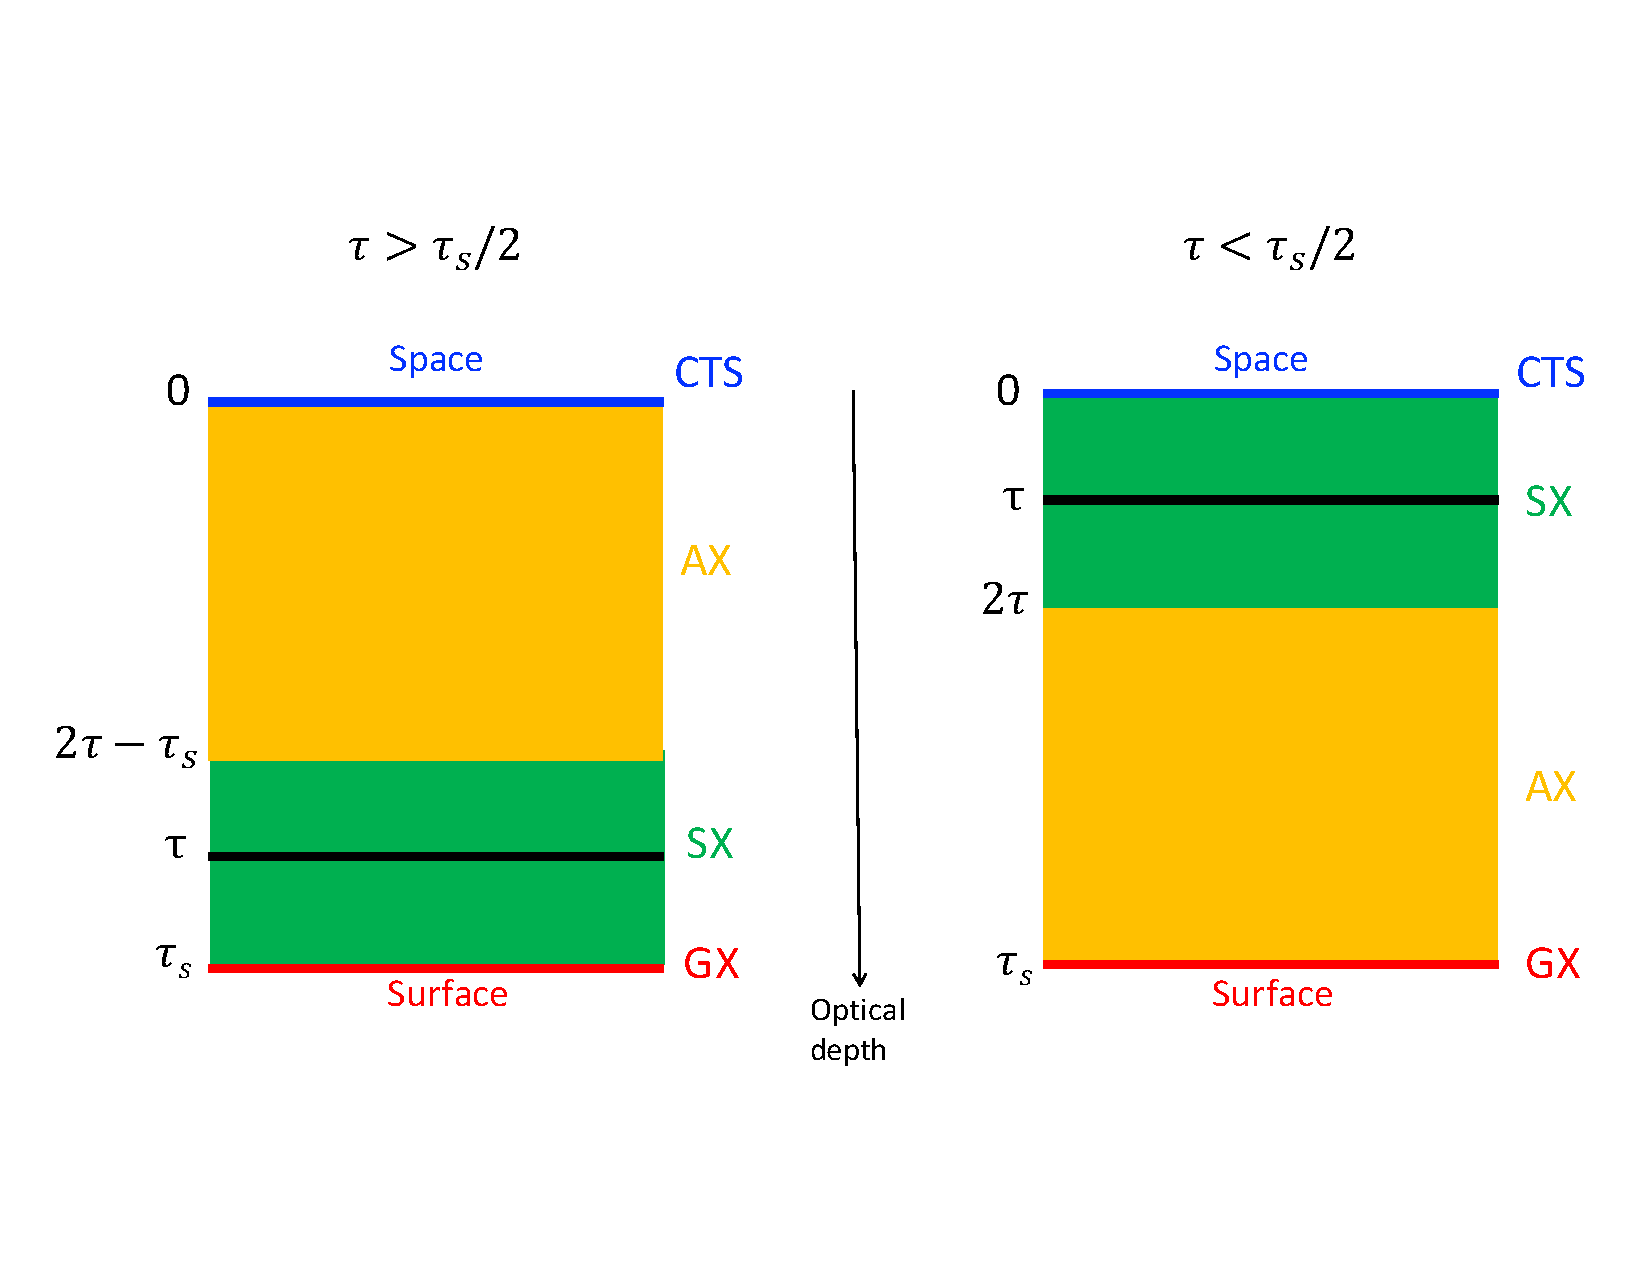
\includegraphics[scale=0.6]{../plots/cts_decomp_cartoon.pdf}
		\caption{Cartoon depicting the atmospheric layers relevant for the different cooling terms in \eqnref{cts_decomp}, relative to a given layer at optical depth $\tau$, for the case where $\tau > \taus/2$ (left) and $\tau<\taus/2$ (right).
		\label{cts_decomp_cartoon}
		}
	\end{center}
\end{figure}

%Figure beta
\begin{figure}[h!]
	\begin{center}
			\includegraphics[scale=0.6]{../plots/beta.pdf}
		\caption{Calculation of $\der{\ln \tauk}{\ln p}$ for various cases, along with $\tauk=1$ levels (averaged in 10 \cminverse\ bins), and the mean and standard deviation of $\der{\ln \tauk}{\ln p}$ restricted to these levels, denoted as $\beta$. The atmospheric profiles fed into RFM were as follows:
					\textbf{(a)}  A modified simple \cotwo\ only atmosphere  with a uniform temperature of 200 K, to eliminate temperature scaling.
					\textbf{(b)}  As in (a) but using our standard simple atmosphere
					\textbf{(c)}  Our  standard simple \htwo\ only atmosphere, except that we impose a uniform 200 K temperature while keeping $q$ unchanged. This yields unphysical \RH\ values, but allows us to eliminate the effect of temperature scaling while preserving the exponential increase of $q$ with depth  
					\textbf{(d)}   As in (c) but using our standard simple atmosphere.
					These panels yield the estimates of $\beta$ found in Table \ref{band_params} and used in our analytical model, and show that our estimates of $\beta$ from \eqnref{tauk_theory} are reasonable in the absence of temperature scaling, but are underestimates in the presence of temperature scaling.
		\label{beta}
		}
	\end{center}
\end{figure}

%Figure cooling_profiles
\begin{figure}[h]
	\begin{center}
			\includegraphics[scale=0.5]{../plots/cooling_profiles.pdf}
		\caption{Spectrally-resolved \htwo\  and \cotwo\ cooling rates, along with the decomposition \eqref{cts_decomp}. The CTS approximations works very well for \htwo\ (at least away from the surface) but not as well for \cotwo. This can be traced to $\beta_{\cotwo} < \beta_{\htwo}$, which also implies that the \cotwo\ weighting function and hence cooling will be weaker and more broadly distributed in the vertical.
		\label{cooling_profiles}
		}
	\end{center}
\end{figure}

%Figure kappa
\begin{figure}[h!]
	\begin{center}
			\includegraphics[scale=0.7]{../plots/kappa.pdf}
		\caption{Reference absorption spectra $\kapparef(k)$, evaluated at (\Tref,\pref)=(300 K, 1 atm), for \htwo\ (left) and \cotwo\ (right). Plotted are \kapparef\ as output from RFM (light gray, dotted), \kapparef\ averaged in 10 \cminverse\ bins (dark gray, thick dashed), and the linear fits \eqnref{kappa_fits} (black, solid). These fits yield the $\kappa_j$ and $l_j$ parameters in Table \ref{band_params}.
		\label{kappa}
		}
	\end{center}
\end{figure}

%Figure tau_rfm_theory
\begin{figure}[h!]
	\begin{center}
			\includegraphics[scale=0.6]{../plots/tau_rfm_theory.pdf}
		\caption{Natural log of optical depth $\tauk$ for 
					\textbf{(a)} \htwo, as output from RFM
					\textbf{(b)} \htwo, as given by \eqnref{tauk_h2o}
					\textbf{(c)} \cotwo, as output from RFM
					\textbf{(d)}	 \cotwo, as given by \eqnref{tauk_co2}.
					These panels show that our analytical formulae \eqnref{tauk_theory} do a remarkably good job of reproducing the gross distribution of optical depth as a function of both wavenumber	and pressure.			
		\label{tau_rfm_theory}
		}
	\end{center}
\end{figure}

%Figure cts_theory
\begin{figure}[h!]
	\begin{center}
			\includegraphics[scale=0.6]{../plots/cts_theory.pdf}
		\caption{Sum of the band-wise heating rates  $\ch_j$ (as calculated via \eqnref{heat_cts3}) for \htwo\ (left) and \cotwo\ (right), along with the heating rate profiles output directly from RFM. The analytic theory does a decent job of estimating the magnitude and general profile shape for both gases. Horizontal dotted line marks the tropopause. See text for further discussion.
		\label{cts_theory}
		}
	\end{center}
\end{figure}

%Figure wvp_check
\begin{figure}[h!]
	\begin{center}
			\includegraphics[scale=0.7]{../plots/wvp_check.pdf}
		\caption{Validation of the formulae \eqnref{WVP2} for water vapor path above a given isotherm $\WVP(T)$ . Profiles of this quantity, in both linear (left) and log (right) axes, are shown for both numerically integrated $\WVP(T)$ derived from the input RFM profile, as well as the profile given by \eqnref{WVP2}.  
		\label{wvp_check}
		}
	\end{center}
\end{figure}


\pagebreak

\bibliographystyle{apa}
\bibliography{/Users/nadir/Dropbox/resources/bibtex_mendeley/library}


\end{document}

